\documentclass{scrartcl}
\usepackage{tikz}
\usetikzlibrary{arrows, automata}
\usepackage{comment}
\usepackage{amsmath}
\usepackage{qtree}
\usepackage{textcomp}
\usepackage{tree-dvips}

\begin{document}

Example 1:
 This is a \TeX file.

 \[
  (f\ast g) = \int_{-\infty}^{\infty} f{\tau} g(t-\tau) \, d\tau
 \]

Example 2:
\textit{As NFA defined on Page 54 of ITC}\\
textbook.\\

% begin math model
$
Q = \{q_1, q_2, q_3, q_4\} \\
\sum = \{0, 1\}\\
F = \{q_4\}\\
q_0 = q_1 \\
\delta = \{
            ((q_1, 0), \{q_1\}), ((q_1, 1), \{q_1, q_2\}), ((q_1, \epsilon), \phi), \\
            ((q_2, 0), \{q_3\}), ((q_2, 1),\phi), ((q_2, \epsilon), \{q_3\}), \\
            ((q_3, 0), \phi), ((q_3, 1), \{q_4\}), ((q_3, \epsilon), \phi), \\
            ((q_4, 0), \{q_4\}), ((q_4, 1), \{q_4\}), ((q_4, \epsilon), \phi)
\} \\
$
%end math model

Transition Function in Table form: \\
\begin{center}
  \begin{tabular}{||c c c c||}
    \hline
    \space  &0      &1              &$\epsilon$    \\[0.5ex]
    \hline
    $q_1$          & \{$q_1$\}      & \{$q_1$, $q_2$\}    &$\phi$        \\
    \hline
    $q_2$          & \{$q_3$\}      & $\phi$              & \{$q_3$\}    \\
    \hline
    $q_3$          & $\phi$         & \{$q_4$\}           & $\phi$       \\
    \hline
    $q_4$          & \{$q_4$\}      & \{$q_4$\}           & $\phi$       \\
    \hline
  \end{tabular}
\end{center}

NFA in pictorial form: \\

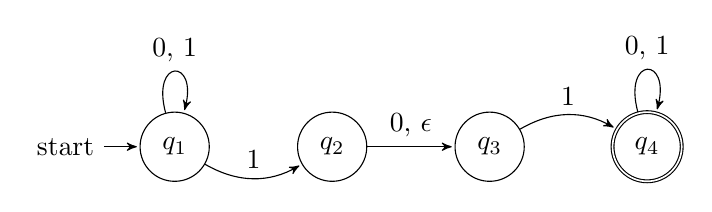
\begin{tikzpicture}[>=stealth',shorten >=1pt, auto, node distance=2cm]
  \node[initial, state]       (q1)                  {$q_1$};
  \node[state]                (q2)[right of=q1]     {$q_2$};
  \node[state]                (q3)[right of=q2]     {$q_3$};
  \node[state, accepting]     (q4)[right of=q3]     {$q_4$};

  \path[->](q1) edge [loop above]    node {0, 1}(q1)
                edge [bend right]    node {1} (q2)
          (q2)  edge                 node {0, $\epsilon$} (q3)
          (q3)  edge [bend left]     node {1} (q4) 
          (q4)  edge [loop above]    node {0, 1} (q4);
\end{tikzpicture}

Example 3:
 \textbf{\textit{DFA, state diagram of machine M}}
\begin{center}
  \begin{tikzpicture}[>=stealth',shorten >=2pt, auto, node distance=5cm]
    %define states in the machine
    \node[initial, state, accepting] (q3) {$q_3$};
    \node[state]  (q2) [above of= q3] {$q_2$};
    \node[state]  (q1) [right of= q2] {$q_1$};
    \node[state]  (q4) [below of=q3] {$q_4$};
    \node[state]  (q5) [right of=q4]  {$q_5$};

    %define the links
    \path[->] (q1) edge[loop above] node{u}  (q1)
                   edge             node{d}  (q2)
              (q2) edge[bend left]  node{u}  (q1)
                   edge             node{d}  (q3)
              (q3) edge[bend left]  node{u}  (q2)
                   edge             node{d}  (q4)
              (q4) edge[bend left]  node{u}  (q3)
                   edge             node{d}  (q5)
              (q5) edge[bend left]  node{u}  (q4)
                   edge[loop above] node{d}  (q5);
  \end{tikzpicture}
\end{center}

Example 4: 
\textbf{Machine DFA has 02 languages and it combine:}\\
\{w$|$ w has at least three a's\}\\
\begin{center}
  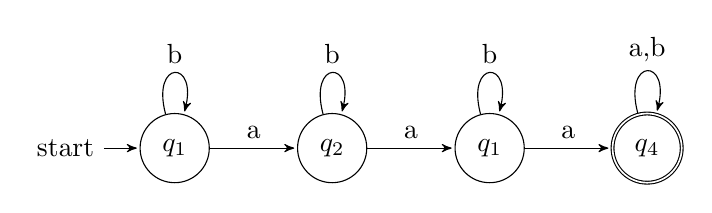
\begin{tikzpicture}[>=stealth',shorten >=1pt,auto, node distance=2cm]
    
    %define the state in the machine
    \node[initial, state] (q1) {$q_1$};
    \node[state]           (q2) [right of=q1] {$q_2$};
    \node[state]           (q3) [right of=q2] {$q_1$};
    \node[state, accepting] (q4) [right of=q3] {$q_4$};

    % define the links
    \path[->](q1)edge[loop above] node {b} (q1)   edge node{a} (q2)
    (q2) edge [loop above] node {b} (q2)
         edge node {a}(q3)
    (q3) edge [loop above] node {b} (q3)
         edge node{a} (q4)
    (q4) edge [loop above] node{a,b} (q4);
  \end{tikzpicture}
\end{center}

\{w$|$ has at least three b's\}\\
\begin{center}
  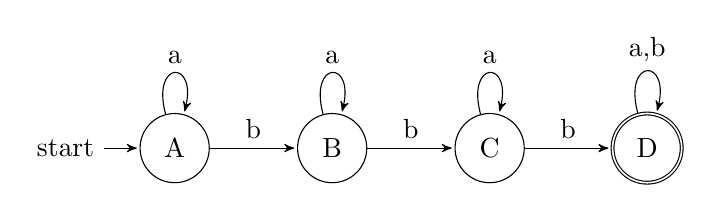
\begin{tikzpicture}[>=stealth', shorten >=1pt, auto, node distance=2cm]

    %define the states in the machine
    \node[initial, state] (q1)  {A};
    \node[state] (q2) [right of=q1] {B};
    \node[state] (q3) [right of=q2] {C};
    \node[state, accepting] (q4) [right of=q3] {D};

    %define the link
    \path[->](q1) edge [loop above] node {a} (q1)
    edge   node {b} (q2)
    (q2) edge [loop above] node {a} (q2)
    edge    node {b} (q3)
    (q3) edge [loop above] node {a} (q4)
         edge  node {b} (q4)
    (q4) edge [loop above] node {a,b} (q4); 
  \end{tikzpicture}
\end{center}

Combining them using the intersection construction for DFA machine:\\
\begin{center}
  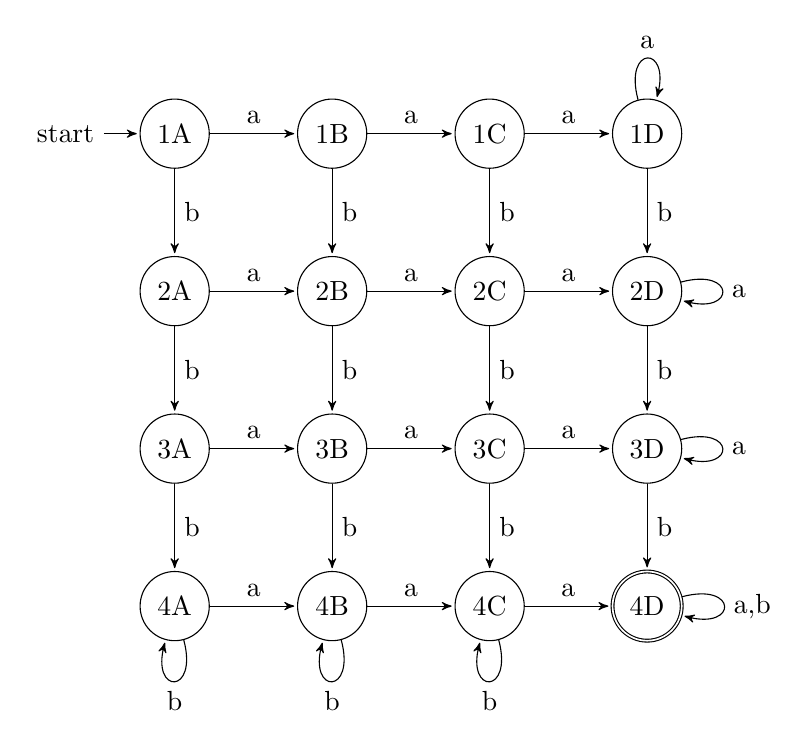
\begin{tikzpicture}[>=stealth', shorten >=1pt, auto, node distance=2cm]
    %define the states in the machine
    \node[initial, state] (q1) {1A};
    \node[state] (q2) [right of=q1] {1B};
    \node[state] (q3) [right of=q2] {1C};
    \node[state] (q4) [right of=q3] {1D};
    \node[state] (q5) [below of=q1] {2A};
    \node[state] (q6) [right of=q5] {2B};
    \node[state] (q7) [right of=q6] {2C};
    \node[state] (q8) [right of=q7] {2D};
    \node[state] (q9) [below of=q5] {3A};
    \node[state] (q10) [right of=q9] {3B};
    \node[state] (q11) [right of=q10] {3C};
    \node[state] (q12) [right of=q11] {3D};
    \node[state] (q13) [below of=q9] {4A};
    \node[state] (q14) [right of=q13] {4B};
    \node[state] (q15) [right of=q14] {4C};
    \node[state, accepting] (q16) [right of=q15] {4D};

    %define the links
    \path[->](q1) edge node {a} (q2) 
                  edge node {b} (q5)
            (q2)  edge node {a} (q3)
                  edge node {b}  (q6)
            (q3)  edge node {a}  (q4)
                  edge node {b}  (q7)
            (q4)  edge [loop above]node {a} (q4)
                  edge node {b}  (q8)
            (q5)  edge node {a}  (q6)
                  edge node {b}  (q9)
            (q6)  edge node {a}  (q7)
                  edge node {b}  (q10)
            (q7)  edge node {a}  (q8)
                  edge node {b}  (q11)
            (q8)  edge [loop right] node {a}(q8)
                  edge node {b}  (q12)
            (q9)  edge node {a}  (q10)
                  edge node {b}  (q13)
            (q10) edge node {a}  (q11)
                  edge node {b}  (q14)
            (q11) edge node {a}  (q12)
                  edge node {b}  (q15)
            (q12) edge[loop right] node{a} (q12)
                  edge node {b}  (q16)
            (q13) edge node {a}  (q14)
                  edge[loop below] node {b}(q13)
            (q14)  edge node {a}  (q15)
                  edge[loop below] node {b}(q14)
            (q15)  edge node {a}  (q16)
                  edge[loop below] node {b}(q15)
            (q16) edge [loop right] node {a,b}(q16);
  \end{tikzpicture}
\end{center}

Regular expression and it diagram DFA:
\textbf{ 1$\sum^*$0}\\
\textbf{\underline{\{w$|$w begin with a 1 and end with a 0\}}}\\

\begin{center}
  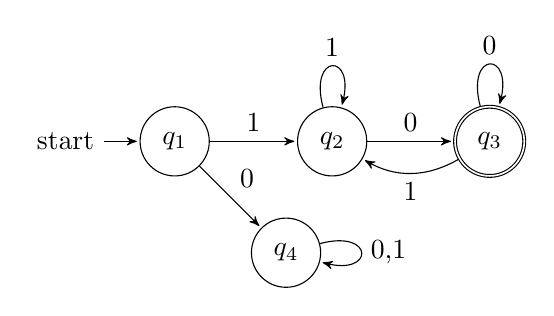
\begin{tikzpicture}[>=stealth', shorten >=1pt, auto, node distance=2cm]

    %define state machine
    \node[initial, state]  (q1) {$q_1$};
    \node[state] (q2) [right of=q1] {$q_2$};
    \node[state, accepting] (q3) [right of=q2] {$q_3$};
    \node[state] (q4) [below right of=q1]{$q_4$};

    %define the links
    \path[->] (q1) edge node{0} (q4)
                   edge node{1} (q2)
              (q2) edge node{0} (q3)
                   edge [loop above] node{1} (q3)
              (q3) edge[loop  above] node{0}(q3)
                  edge [bend left] node{1}(q2)
              (q4) edge [loop right] node{0,1} (q4);
                
  \end{tikzpicture}
\end{center}

\textbf{\{w $|$ w = $w^R$,. that is, w is a palindrome\}}\\
\begin{center}
      S $\rightarrow $ 0S0 $|$ 1S1 $|$ 0 $|$ 1 $|$ $\epsilon$ \\
\end{center}
\textit{Informal description: We begin by pushing the symbols read onto the stack. At each point we will nondeterministically guess if the middle of the string has been  reached or if  the next symbol read is the middle of the string and will not  be put on  the stack. Then we  pop off the symbols from the stack if they match the input symbol read. If the symbol popped are exactly the same symbols that were pushed on earlier and the stack empties as the input is finished, ten accept. Otherwise, reject.}\\

\begin{center}
  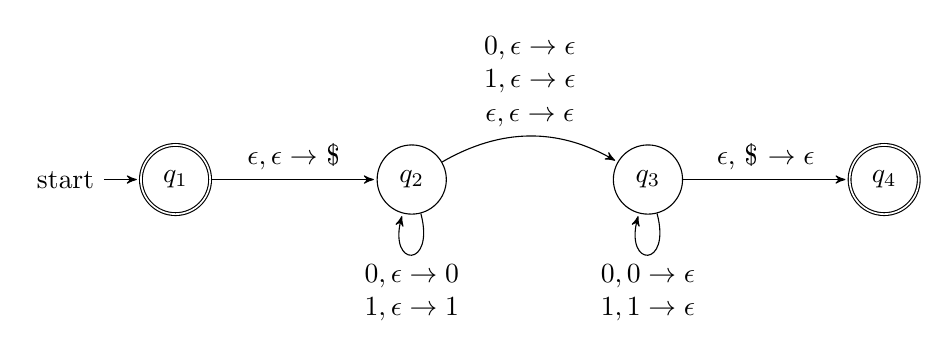
\begin{tikzpicture}[>=stealth',shorten >=1pt,auto,node distance=3cm]
% define the states in the machine
  \node[initial,state, accepting] 	(q1)      				{$q_1$};
  \node[state]  	(q2) [right of=q1]           	{$q_2$};
  \node[state]         		(q3) [right of=q2]  	{$q_3$};
  \node[state, accepting]    (q4) [right of=q3]  	{$q_4$};

     % define the links
  \path[->] (q1)  edge  	node {$\epsilon,\epsilon \rightarrow $ \$  }	(q2)
             
  (q2) edge [loop below, align=center]  	node {$0, \epsilon \rightarrow 0$ \\ $1, \epsilon \rightarrow 1$ } 	(q2)
       edge [bend left, align=center] node {$0, \epsilon \rightarrow \epsilon$ \\ $1, \epsilon \rightarrow \epsilon$ \\ $\epsilon, \epsilon \rightarrow \epsilon$}  	(q3)
  (q3) edge [loop below, align=center]  node {$0, 0 \rightarrow \epsilon$ \\ $1, 1 \rightarrow \epsilon$} 	(q3)
       edge   node {$\epsilon$, \$ $\rightarrow \epsilon $} (q4);

  \end{tikzpicture}
\end{center}

%Regular expression
\textbf{Example 4: D=\{w$|$w contains an even number of a's and odd number of b's and does not contain the substring ab\}}\\

\begin{center}
 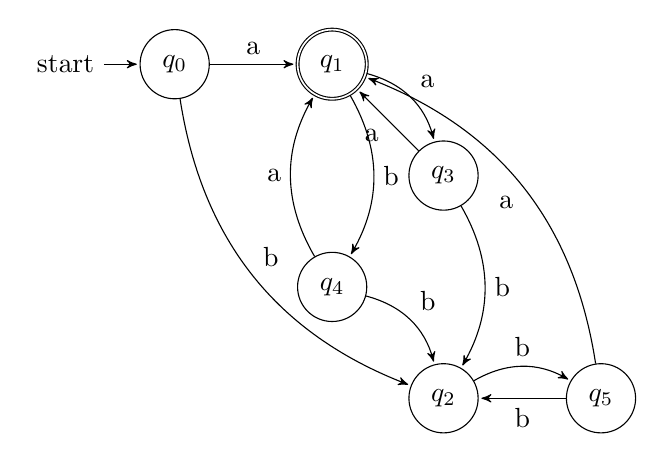
\begin{tikzpicture}[>=stealth',shorten >=1pt,auto,node distance=2cm]
 
% define the states in the machine
  \node[initial, state]    (q0) 
{$q_0$};
  \node[state, accepting]   (q1)   [right of=q0]  	    
{$q_1$};
\node[state]    (q3)  [below right of=q1]
{$q_3$};
  
\node[state]    (q4)  [ below left of=q3]
{$q_4$};
 \node[state]   (q2)   [below right of=q4]  	    
{$q_2$};
 \node[state]   (q5)   [ right of=q2]  	    
{$q_5$};
  
% define the links
  \path[->] (q0) edge  node {a} (q1)
             edge [bend right] node {b} (q2)
        (q1) edge  [bend left] node {a} (q3)
             edge  [bend left] node {b} (q4)
        (q2) edge [bend left]  node {b}  (q5)
             
        (q3) edge   node {a}  (q1)
             edge  [bend left] node {b}   (q2)
        (q4) edge [bend left]  node {a} (q1)
             edge  [bend left] node {b} (q2)
        (q5) edge  [bend right] node {a} (q1)
             edge   node {b}  (q2);
                
                                              
 \end{tikzpicture}
\end{center}
\textbf{ regular expression:   $(aa|ba|bb)^*(a|b)$ }\\

\textbf{4b. \{w$|$ w contains the substring 0101, e.x. w = x0101y for some x and y\}}\\

\begin{center}
 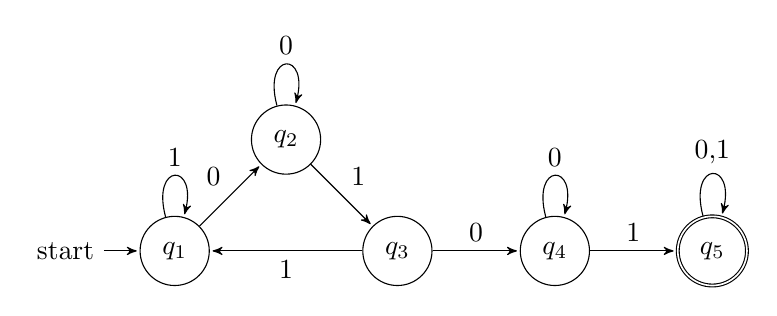
\begin{tikzpicture}[>=stealth',shorten >=1pt,auto,node distance=2cm]
 
% define the states in the machine
  \node[initial, state]     (q1) 
{$q_1$};
  \node[state]   (q2)   [above right of=q1]  	    
{$q_2$};
  \node[state]   (q3)   [below right of=q2]
{$q_3$};
  \node[state]   (q4)   [right of=q3]
{$q_4$};
  \node[state, accepting]   (q5)  [right of=q4] 
{$q_5$};
  
% define the links
  \path[->] (q1) edge [loop above] node {1} 	(q1)
             edge               node {0} 	(q2)
        (q2) edge  [loop above] node {0}  (q2)
             edge              node {1} (q3)
        (q3) edge              node {1} (q1)
             edge               node {0}  (q4)
        (q4) edge  [loop above] node {0}  (q4)
             edge              node {1}   (q5)
        (q5) edge  [loop above] node {0,1} (q5);
                    
      
 \end{tikzpicture}
\end{center}


\textbf{4c. \{ w$|$ w starts with 0 and has odd length, or starts with 1 and has even length\} }\\

\begin{center}
 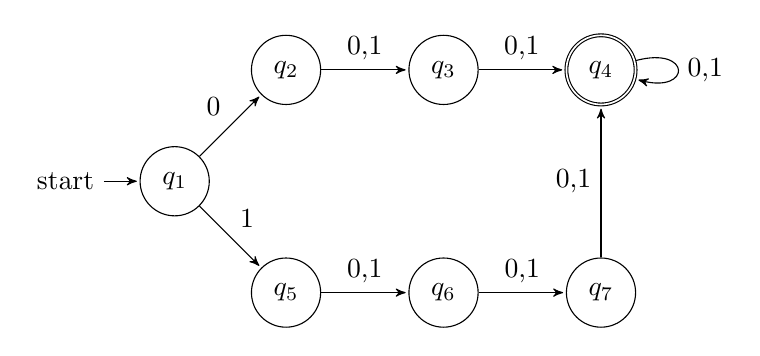
\begin{tikzpicture}[>=stealth',shorten >=1pt,auto,node distance=2cm]
 
% define the states in the machine
  \node[initial, state]     (q1) 
{$q_1$};
  \node[state]   (q2)   [above right of=q1]  	    
{$q_2$};
  \node[state]   (q3)   [right of=q2]
{$q_3$};
  \node[state, accepting]   (q4)   [right of=q3]
{$q_4$};
  \node[state]   (q5)   [below right of=q1]
{$q_5$};
  \node[state]   (q6)   [right of=q5]
{$q_6$};
  \node[state]   (q7)   [right of=q6]
{$q_7$};
  
  
% define the links
  \path[->] (q1) edge     node {0} 	(q2) 
                 edge     node {1}   (q5)   
        (q2) edge         node {0,1}     (q3)    
        (q3) edge         node {0,1}       (q4)   
        (q4) edge  [loop right]  node {0,1}  (q4)
        (q5) edge         node {0,1}  (q6)
        (q6) edge         node {0,1}  (q7)
        (q7) edge         node {0,1}  (q4);
                               
 \end{tikzpicture}
\end{center}
\textbf{4c.  $(0\cup 1\sum)(\sum\sum)^*$ }  in regular expression\\

\textbf{Example 5. Give an NFA recognizing the language $(01\cup 001 \cup 010)^*$}\\

\begin{center}
 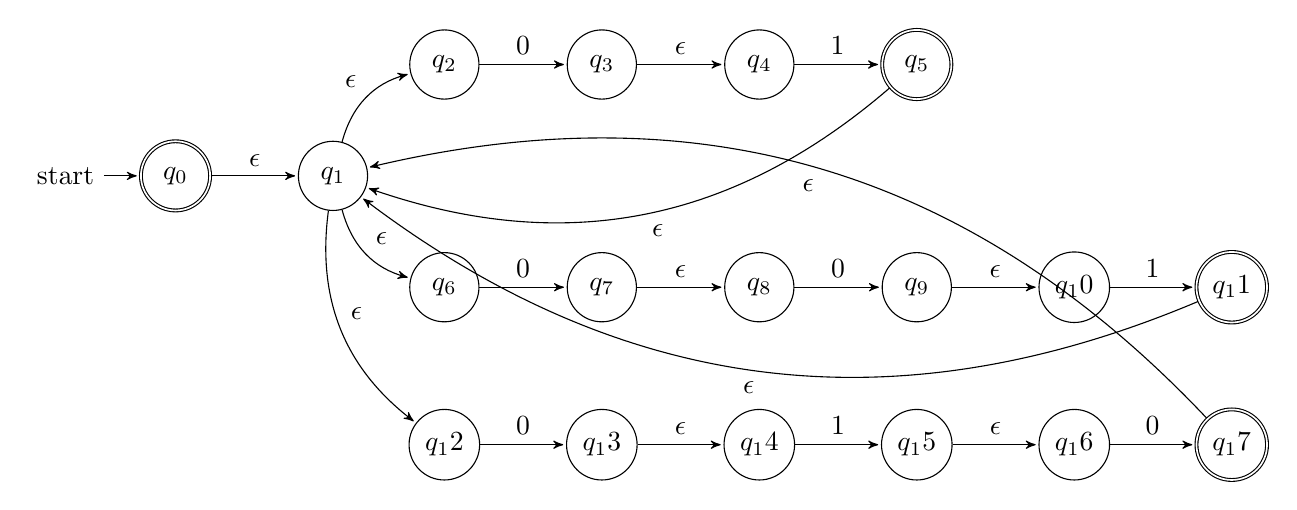
\begin{tikzpicture}[>=stealth',shorten >=1pt,auto,node distance=2cm]
 
% define the states in the machine
  \node[initial, state, accepting]    (q0) 
{$q_0$};
  \node[state]   (q1)   [right of=q0]  	    
{$q_1$};
  \node[state]    (q2)  [above right of=q1]
{$q_2$}; 
 \node[state]    (q3)  [right of=q2]
{$q_3$};
 \node[state]    (q4)  [right of=q3] 
{$q_4$};
  \node[state, accepting]   (q5)   [right of=q4]  	    
{$q_5$};
  \node[state]    (q6)  [below right of=q1]
{$q_6$}; 
 \node[state]    (q7)  [right of=q6]
{$q_7$};
 \node[state]    (q8)  [right of=q7]
{$q_8$};
  \node[state]   (q9)   [right of=q8]  	    
{$q_9$};
  \node[state]    (q10)  [right of=q9]
{$q_10$}; 
 \node[state, accepting]    (q11)  [right of=q10]
{$q_11$};
 \node[state]    (q12)  [below of=q6]
{$q_12$};
  \node[state]   (q13)   [right of=q12]  	    
{$q_13$};
  \node[state]    (q14)  [right of=q13]
{$q_14$}; 
 \node[state]    (q15)  [right of=q14]
{$q_15$};
 \node[state]    (q16)  [right of=q15]
{$q_16$};
 \node[state, accepting]    (q17)  [right of=q16]
{$q_17$};
 
% define the links
  \path[->] (q0) edge  node {$\epsilon$} (q1)
             
        (q1) edge  [bend left] node {$\epsilon$} (q2)
             edge  [bend right] node {$\epsilon$} (q6)
             edge  [bend right] node {$\epsilon$} (q12)
        (q2) edge   node {0}  (q3)
        (q3) edge   node {$\epsilon$}  (q4)
        (q4) edge   node {1}  (q5)
        (q5) edge   [bend left] node {$\epsilon$} (q1)
        (q6) edge   node {0}  (q7)
        (q7) edge   node {$\epsilon$} (q8)
        (q8) edge   node {0}   (q9)
        (q9) edge   node {$\epsilon$} (q10)
        (q10) edge  node {1}  (q11)
        (q11) edge  [bend left] node {$\epsilon$} (q1)
        (q12) edge  node {0}    (q13)
        (q13) edge  node {$\epsilon$} (q14)
        (q14) edge  node {1}   (q15)
        (q15) edge  node {$\epsilon$} (q16)
        (q16) edge  node {0}  (q17)
        (q17) edge  [bend right] node {$\epsilon$} (q1);        
                                                   
 \end{tikzpicture}
\end{center}

\textbf{5a. \{w $|$ w starts and ends with the same symbol\}}\\
\begin{center}
S $\rightarrow$ 0T0 $|$ 1T1 $|$ 0 $|$ 1\\
T $\rightarrow$ 0T $|$ 1T $|$ $\epsilon$ \\
\end{center}

\textit{ Informal description: We will nondeterministically guess if the  string has  only one symbol in which  case we accept it without using the stack. Then we will read every other symbol and nondeterministically guess if that is the last symbol read. If the last symbol read then matches the symbol on the stack and there is no more input we accept. Otherwise we reject. }\\

\begin{center}
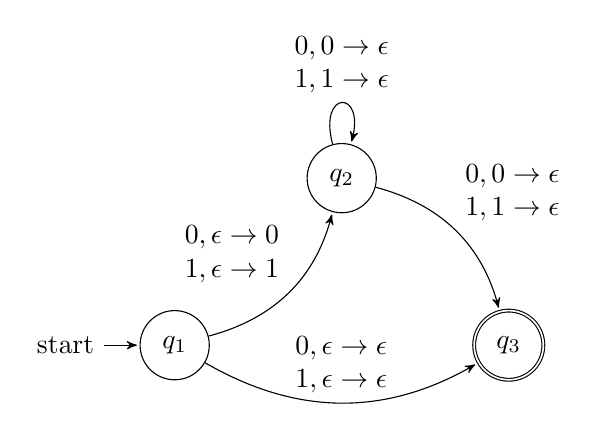
\begin{tikzpicture}[>=stealth',shorten >=1pt,auto,node distance=3cm]
% define the states in the machine
  \node[initial,state] 	(q1)      				{$q_1$};
  \node[state]  	(q2) [above right of=q1]           	{$q_2$};
  \node[state, accepting]     (q3) [below right of=q2]  	{$q_3$};

% define the links
  \path[->] (q1)  edge [bend right, align=center]	node {$0, \epsilon \rightarrow 0$ \\ $1, \epsilon \rightarrow 1$} 	(q2)
             edge [bend right, align=center] node {$0, \epsilon \rightarrow \epsilon $ \\ $1, \epsilon \rightarrow \epsilon$} (q3)
        (q2) edge [loop above, align=center]  	node {$0, 0 \rightarrow \epsilon$ \\ $1, 1 \rightarrow \epsilon$} 	(q2)
             edge [bend left, align=center]	node {$0, 0 \rightarrow \epsilon$ \\ $1, 1 \rightarrow \epsilon$}  	(q3);
        
\end{tikzpicture}
\end{center}

\textbf{5b.  \{ w$|$ w has length at least 3 and third symbol is a 0\}}\\

\begin{center}
 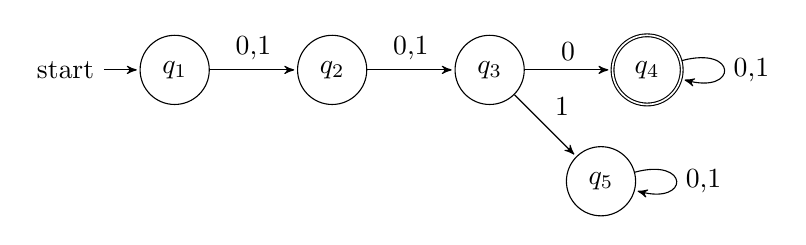
\begin{tikzpicture}[>=stealth',shorten >=1pt,auto,node distance=2cm]
 
% define the states in the machine
  \node[initial, state]     (q1) 
{$q_1$};
  \node[state]   (q2)   [right of=q1]  	    
{$q_2$};
  \node[state]   (q3)   [right of=q2]
{$q_3$};
  \node[state, accepting]   (q4)   [right of=q3]
{$q_4$};
  \node[state]   (q5)   [below right of=q3]
{$q_5$};
  
  
% define the links
  \path[->] (q1) edge     node {0,1} 	(q2)    
        (q2) edge         node {0,1}     (q3)
             
        (q3) edge         node {0}       (q4)
             edge         node {1}       (q5)
        (q4) edge  [loop right]  node {0,1}  (q4)
        (q5) edge  [loop right]  node {0,1}  (q5);
                               
 \end{tikzpicture}
\end{center}

\textbf{5c. \{w $|$ the length of w is odd and its middle symbol is 0's\}}\\

S $\rightarrow$ 0 $|$  0S0 $|$ 0S1 $|$ 1S0 $|$ 1S1 \\
\textit{Formal description: The PDA scans across the string and push the symbol onto the stack. At some point it nondeterministically guesses where the middle is. It looks at the middle symbol. If that symbol is a 1, it rejects. Otherwise, it scans the rest of the string, and for each character scanned, it pops one element off of its stack. If the stack is empty when it finishes reading the input (ex: it correctly guessed the middle then it accepts.}\\

\begin{center}
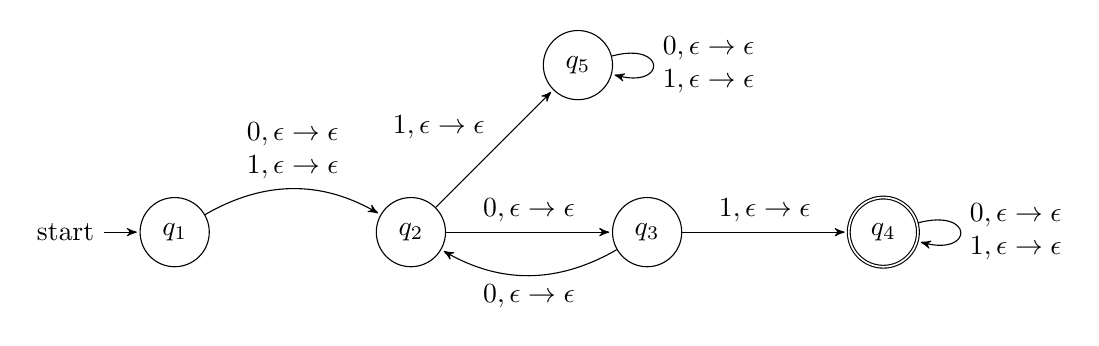
\begin{tikzpicture}[>=stealth',shorten >=1pt,auto,node distance=3cm]
% define the states in the machine
  \node[initial,state] 	(q1)      				{$q_1$};
  \node[state]  	(q2) [right of=q1]           	{$q_2$};
  \node[state]         		(q3) [right of=q2]  	{$q_3$};
  \node[state, accepting]    (q4) [right of=q3]  	{$q_4$};
  \node[state]    (q5) [above right of=q2]  	{$q_5$};

% define the links
  \path[->] (q1)  edge [bend left, align=center] 	node {$0,\epsilon \rightarrow \epsilon$ \\ $1, \epsilon \rightarrow \epsilon$} 	(q2)
        (q2) edge  	node {$0, \epsilon \rightarrow \epsilon$} 	(q3)
             edge 	node {$1, \epsilon \rightarrow \epsilon$}  	(q5)
        (q3) edge [bend left]  	node {$0, \epsilon \rightarrow \epsilon$} 	(q2)
             edge   node {$1, \epsilon \rightarrow \epsilon$} (q4)
         (q4) edge [loop right, align=center] node {$0, \epsilon \rightarrow \epsilon $ \\ $1, \epsilon \rightarrow \epsilon $} (q4)     
         (q5) edge [loop right, align=center] node {$0, \epsilon \rightarrow \epsilon$ \\ $1, \epsilon \rightarrow \epsilon$} (q5);
             
\end{tikzpicture}
\end{center}
\textbf{ Example 6.Modify machine M2 to recognize even number of 0s and draw the state diagram.}\\
$\sum$ =\{0\}\\
$\Gamma$=\{0,x,\textvisiblespace\}\\
$\delta$ transition function as TM state diagram:\\
\begin{center}
\begin{tikzpicture}[>=stealth',shorten >=3pt,auto,node distance=5cm]
% define the states in the machine
  \node[initial,state] 	(q1)      				{$q_1$};
  \node[state]  	(q2) [right of=q1]           	{$q_2$};
  \node[state]         		(q3) [right of=q2]  	{$q_3$};
  \node[state]    (q4) [below of=q3]  	{$q_4$};
  \node[state]    (q5) [above right of=q2]  	{$q_5$};
  \node[state]         		(q6) [below of=q1]  	{$q_accept$};

% define the links
  \path[->]  (q1) edge  node {0 $\rightarrow \textvisiblespace$, R} (q2)
             edge  node {$\textvisiblespace \rightarrow$ R} (q6)
             (q2)  edge [loop above] node {x $\rightarrow$ R} 	(q2)
             edge   node {0 $\rightarrow$x,R} (q3)
             edge  [bend left] node {$\textvisiblespace \rightarrow R$} (q6)
        (q3) edge [loop right]  	node {x $\rightarrow$ R} 	(q3)
             edge 	[bend left] node {0 $\rightarrow$ R}  	(q4)
             edge  [bend right] node {$\textvisiblespace \rightarrow $ L} (q5)
        (q4) edge [loop right]  	node {x $\rightarrow$ R} 	(q4)
             edge   node {0 $\rightarrow$ x, R} (q3)
         (q5) edge [loop above, align=center] node {$0  \rightarrow $ L\\ $x \rightarrow $ L} (q5)
             edge  [bend right] node{$\textvisiblespace \rightarrow R$} (q2);
             
\end{tikzpicture}
\end{center}

\textbf{\textit{b. The folowing are DFA for two languages: }}\\
\{w$|$ w starts with and a\}\\

\begin{center}
 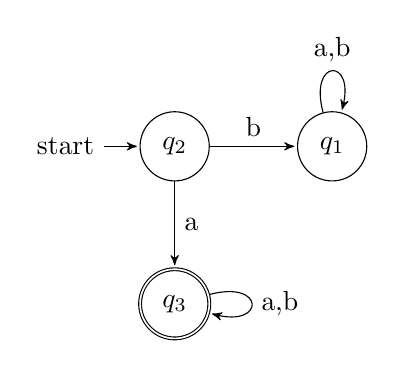
\begin{tikzpicture}[>=stealth',shorten >=1pt,auto,node distance=2cm]
 
% define the states in the machine
  \node[initial, state]  	(q2)   	    {$q_2$};
  \node[state]  (q1)  [right of=q2]   {$q_1$};
  \node [state, accepting]   (q3) [below of=q2]  {$q_3$};
  

% define the links
  \path[ ->] (q2) edge   node {b} (q1) 
              edge   node {a}     (q3)
         (q1) edge [loop above]  node {a,b}  (q1)
        (q3) edge    [loop right] node {a,b} (q3);
        
              
 \end{tikzpicture}
\end{center}

\{w$|$ w has at most one b\}\\
\begin{center}
 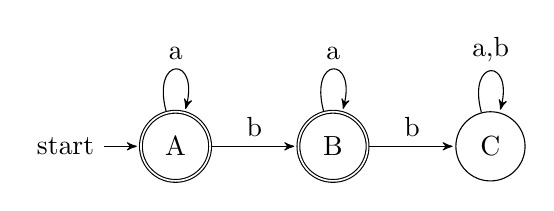
\begin{tikzpicture}[>=stealth',shorten >=1pt,auto,node distance=2cm]
 
% define the states in the machine
  \node[initial, state, accepting]   (q1) 
{A};
  \node[state, accepting]  	(q2)   [right of=q1]  	    
{B};
  \node[state] 	(q3)   [ right of=q2]    				{C};
  
% define the links
  \path[->] (q1) edge [loop above] node {a} 	(q1)
             edge            node {b} 	(q2)
        (q2) edge  [loop above] node {a} (q2) 
             edge              node {b} (q3)  
        (q3) edge [loop above] node {a,b}	(q3);               
                
 \end{tikzpicture}
\end{center}

Combining them using the intersection construction gives the folowing DFA: \\
 
 \begin{center}
 \begin{tikzpicture}[>=stealth',shorten >=1pt,auto,node distance=2cm]
 
% define the states in the machine
  
  \node[initial, state]   (q4) 
{2A};
  \node[state]  	(q5)   [right of=q4]  	    
{2B};
  \node[state] 	(q6)   [ right of=q5]    	
{2C};
  \node[state]   (q1)   [above of=q3]              
{1A};
  \node[state]  	(q2)   [right of=q1]  	    
{1B};
  \node[state] 	(q3)   [right of=q2]    				{1C};
  
  \node[state, accepting]   (q7)    [below of=q4]
{3A};
  \node[state, accepting]  	(q8)   [right of=q7]  	    
{3B};
  \node[state] 	(q9)   [right of=q8]    				{3C};
  
 

% define the links
  \path[->] (q1) edge [loop above]  node {a} 	(q1)
             edge          node {b} 	(q2)
        (q2) edge  [loop above]   node {a}    (q3) 
             edge          node {b} (q3)  
        (q3) edge  [loop right]     node {a,b}   (q3)
             
        (q4) edge         node {b}  (q2)
             edge      node    {a}   (q7)  
        (q5) edge       node {b} 	(q3)
             edge             node {a} 	(q8)
        (q6) edge           node {b}    (q3) 
             edge              node {a} (q9)  
        (q7) edge           node {b}	   (q8)
             edge  [loop below]   node {a}  (q7)
        (q8) edge         node {b}  (q9)
             edge  [loop below]   node {a}   (q8)
        (q9) edge  [loop right]  node {a,b}  (q9);
        
        
 \end{tikzpicture}
\end{center}

\textbf{\textit{c. The folowing are DFA for two languages: }}\\
\{w$|$ w has an odd number of a's\}\\

\begin{center}
 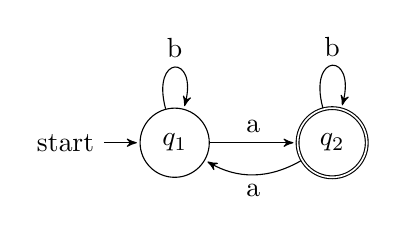
\begin{tikzpicture}[>=stealth',shorten >=1pt,auto,node distance=2cm]
 
% define the states in the machine
  \node[initial, state]   (q1) 
{$q_1$};
  \node[state, accepting]  	(q2)   [right of=q1]  	    
{$q_2$};
  

% define the links
  \path[->] (q1) edge [loop above] node {b} 	(q1)
             edge            node {a} 	(q2)
        (q2) edge  [loop above] node {b} (q2) 
              edge [bend left]  node {a}     (q1); 
                    
 \end{tikzpicture}
\end{center}

\{w$|$ w ends with a b\}\\
\begin{center}
 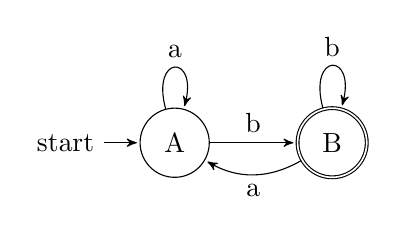
\begin{tikzpicture}[>=stealth',shorten >=1pt,auto,node distance=2cm]
 
% define the states in the machine
  \node[initial, state]   (q1) 
{A};
  \node[state, accepting]  	(q2)   [right of=q1]  	    
{B};
  

% define the links
  \path[->] (q1) edge [loop above] node {a} 	(q1)
             edge            node {b} 	(q2)
        (q2) edge  [loop above] node {b} (q2) 
              edge [bend left]  node {a}     (q1);   
              
 \end{tikzpicture}
\end{center}

Combining them using the intersection construction gives the folowing DFA: \\
\begin{center}
 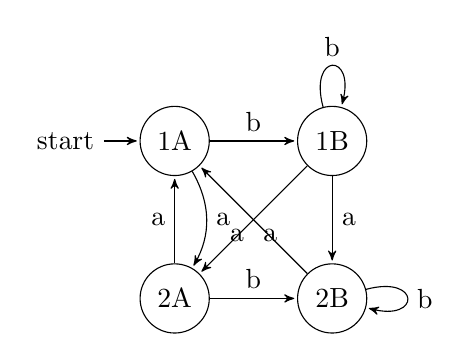
\begin{tikzpicture}[>=stealth',shorten >=1pt,auto,node distance=2cm]
 
% define the states in the machine
  
  \node[initial, state]   (q1) 
{1A};
  \node[state]  	(q2)   [right of=q1]  	    
{1B};
  \node[state] 	(q3)   [ below of=q1]    	
{2A};
  \node[state]   (q4)   [right of=q3]              
{2B};
 

% define the links
  \path[->] (q1) edge   node {b} 	(q2)
             edge  [bend left]     node {a} 	(q3)
        (q2) edge  [loop above]   node {b}    (q2) 
             edge          node {a} (q4) 
             edge         node  {a}  (q3) 
        (q3) edge         node {b}   (q4)
             edge        node  {a}   (q1)
             
        (q4) edge         node {a}  (q1)
             edge  [loop right]    node    {b}   (q4);  
       
 \end{tikzpicture}
\end{center}
\textbf{7. Use theorem 1.39 to convert the folowing to nondeterministic finite automata to equivalent deterministic finite automata.}\\
\textbf{a. }\\

\begin{center}
 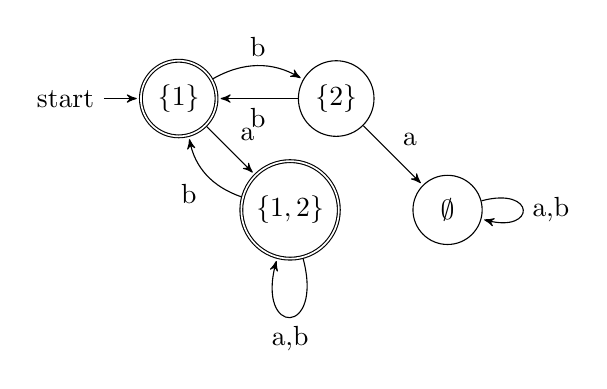
\begin{tikzpicture}[>=stealth',shorten >=1pt,auto,node distance=2cm]
 
% define the states in the machine
  \node[initial, state, accepting]    (q0) 
{$\{1\}$};
  \node[state]   (q1)   [right of=q0]  	    
{$\{2\}$};
\node[state, accepting]    (q2)  [below right of=q0]
{$\{1,2\}$};
  
\node[state]    (q3)  [right of=q2]
{$\emptyset$};
 
% define the links
  \path[->] (q0) edge [bend left] node {b} (q1)
             edge  node {a} (q2)
        (q1) edge   node {b} (q0)
             edge   node {a} (q3)
        (q2) edge  [bend left] node {b}  (q0)
             edge [loop below] node {a,b} (q2)
        (q3) edge [loop right]  node {a,b}  (q3);
                                              
 \end{tikzpicture}
\end{center}

\textbf{b.}\\

\begin{center}
 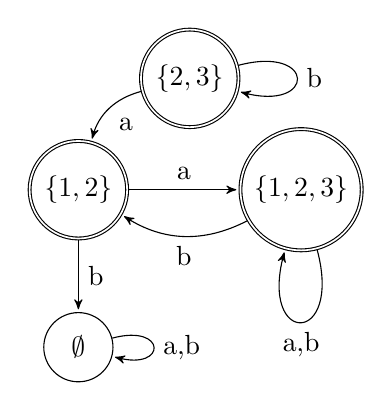
\begin{tikzpicture}[>=stealth',shorten >=1pt,auto,node distance=2cm]
 
% define the states in the machine
  \node[state, accepting]    (q0) 
{$\{1,2\}$};
  \node[state, accepting]   (q1)   [above right of=q0]  	    
{$\{2,3\}$};
\node[state, accepting]    (q2)  [below right of=q1]
{$\{1,2,3\}$};
  
\node[state]    (q3)  [below of=q0]
{$\emptyset$};
 
% define the links
  \path[->] (q0) edge  node {a} (q2)
             edge  node {b} (q3)
        (q1) edge [loop right]  node {b} (q1)
             edge  [bend right] node {a} (q0)
        (q2) edge  [bend left] node {b}  (q0)
             edge [loop below] node {a,b} (q2)
        (q3) edge [loop right]  node {a,b}  (q3);
                                              
 \end{tikzpicture}
\end{center}

\textbf{ c. \{ w$|$ w is any string except 11 and 111\}}\\

\begin{center}
 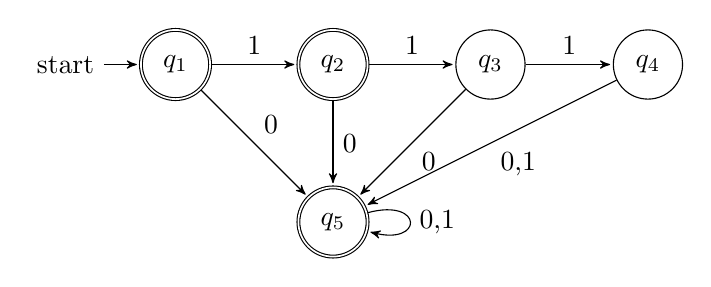
\begin{tikzpicture}[>=stealth',shorten >=1pt,auto,node distance=2cm]
 
% define the states in the machine
  \node[initial, state, accepting]     (q1) 
{$q_1$};
  \node[state, accepting]   (q2)   [right of=q1]  	    
{$q_2$};
  \node[state]   (q3)   [right of=q2]
{$q_3$};
  \node[state]   (q4)   [right of=q3]
{$q_4$};
  \node[state, accepting]   (q5)   [below of=q2]
{$q_5$};
  
% define the links
  \path[->] (q1) edge     node {1} 	(q2)
             edge         node {0}   (q5)
        (q2) edge         node {1}   (q3)
             edge         node {0}   (q5)  
        (q3) edge         node {1}   (q4)
             edge         node {0}   (q5)
        (q4) edge         node {0,1}  (q5)
        (q5) edge [loop right]  node {0,1}   (q5);
        
                               
 \end{tikzpicture}
\end{center}

\textbf{8. Use the construction in the proof of Theorem 1.45 to give the state diagrams of DFA recognizing the union of the languages described in.}\\

\textbf{a.  Exercise 1.6a and 1.6b}\\

\begin{center}
 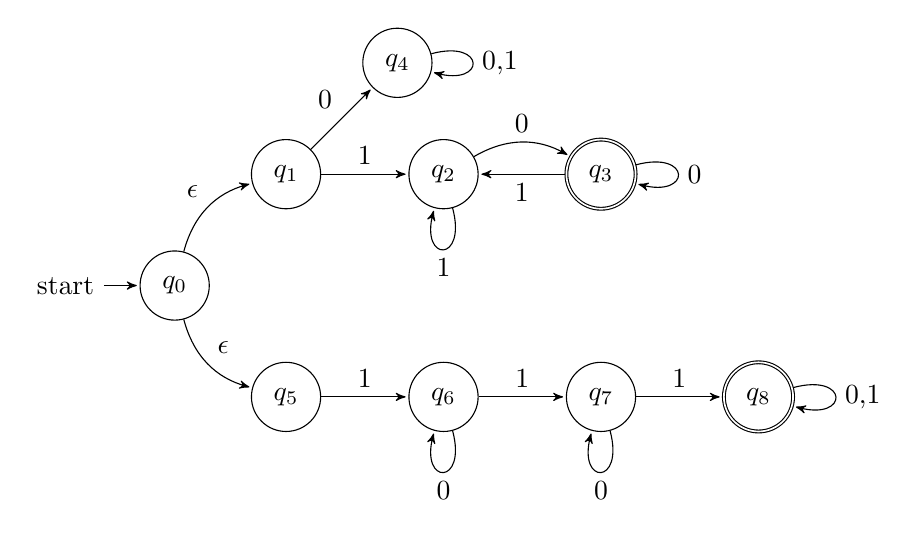
\begin{tikzpicture}[>=stealth',shorten >=1pt,auto,node distance=2cm]
 
% define the states in the machine
  \node[initial, state]    (q0) 
{$q_0$};
  \node[state]   (q1)   [above right of=q0]  	    
{$q_1$};
\node[state]    (q2)  [right of=q1]
{$q_2$};
  \node[state, accepting]   (q3)   [right of=q2]  	    
{$q_3$};
\node[state]    (q4)  [above right of=q1]
{$q_4$};
  \node[state]   (q5)   [below right of=q0]  	    
{$q_5$};
\node[state]    (q6)  [right of=q5]
{$q_6$};
  \node[state]   (q7)   [right of=q6]  	    
{$q_7$};
\node[state, accepting]    (q8) [right of=q7]
{$q_8$};
  
% define the links
  \path[->] (q0) edge [bend left] node {$\epsilon$} (q1)
             edge  [bend right] node {$\epsilon$}  (q5)   
        (q1) edge   node {1} (q2)
             edge   node {0} (q4)
        (q2) edge  [bend left] node {0}  (q3)
             edge  [loop below] node {1}   (q2)
        (q3) edge  [loop right] node {0}  (q3)
             edge   node {1}       (q2)
        (q4) edge  [loop right]  node {0,1}  (q4)
        
        (q5) edge  node {1}  (q6)
        (q6) edge  node {1}  (q7)
             edge  [loop below] node {0} (q6)
        (q7) edge  node {1} (q8)
             edge  [loop below] node {0}  (q7)
        (q8) edge  [loop right] node {0,1} (q8); 
                                         
 \end{tikzpicture}
\end{center}

\textbf{b. Exercise 1.6 c and 1.6f }\\

\begin{center}
 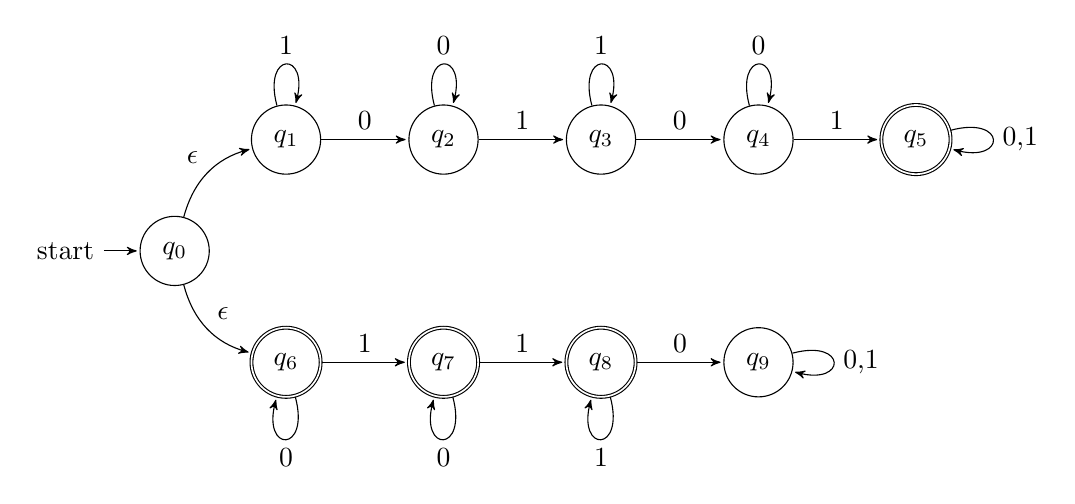
\begin{tikzpicture}[>=stealth',shorten >=1pt,auto,node distance=2cm]
 
% define the states in the machine
  \node[initial, state]    (q0) 
{$q_0$};
  \node[state]   (q1)   [above right of=q0]  	    
{$q_1$};
  \node[state]    (q2)  [right of=q1]
{$q_2$};
  \node[state]   (q3)   [right of=q2]  	    
{$q_3$};
  \node[state]   (q4)  [right of=q3]
{$q_4$};
  \node[state, accepting]   (q5)   [right of=q4]  	    
{$q_5$};
  \node[state, accepting]    (q6)  [ below right of=q0]
{$q_6$};
  \node[state, accepting]   (q7)   [right of=q6]  	    
{$q_7$};
  \node[state, accepting]    (q8) [right of=q7]
{$q_8$};
  \node[state]    (q9) [right of=q8]
{$q_9$};
  
% define the links
  \path[->] (q0) edge [bend left] node {$\epsilon$} (q1)
             edge  [bend right] node {$\epsilon$}  (q6)   
        (q1) edge   node {0} (q2)
             edge [loop above]  node {1} (q1)
        (q2) edge   node {1}  (q3)
             edge  [loop above] node {0}   (q2)
        (q3) edge  [loop above] node {1}  (q3)
             edge   node {0}       (q4)
        (q4) edge  [loop above]  node {0}  (q4)
             edge   node {1}   (q5)
        (q5) edge  [loop right] node {0,1}  (q5)
        (q6) edge  node {1}  (q7)
             edge  [loop below] node {0} (q6)
        (q7) edge  node {1} (q8)
             edge  [loop below] node {0}  (q7)
        (q8) edge  [loop below] node {1} (q8)
             edge     node {0}  (q9)
        (q9) edge [loop right] node {0,1} (q9);
                                         
 \end{tikzpicture}
\end{center}

\textbf{c.  The empty state}\\

\begin{center}
 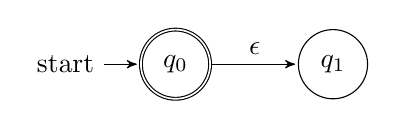
\begin{tikzpicture}[>=stealth',shorten >=1pt,auto,node distance=2cm]
 
% define the states in the machine
  \node[initial, state, accepting]    (q0) 
{$q_0$};
  \node[state]   (q1)   [right of=q0]  	    
{$q_1$};

  
% define the links
  \path[->] (q0) edge  node {$\epsilon$} (q1);
                                              
 \end{tikzpicture}
\end{center}

\textbf{\underline{d.}}\\
\{w$|$ w is string accept a and b\}\\

\begin{center}
 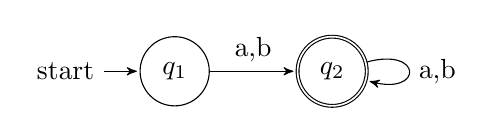
\begin{tikzpicture}[>=stealth',shorten >=1pt,auto,node distance=2cm]
 
% define the states in the machine
  \node[initial, state]     (q1) 
{$q_1$};
  \node[state, accepting]   (q2)   [right of=q1]  	    
{$q_2$};
  
  
% define the links
  \path[->] (q1) edge      node {a,b} 	(q2)
             
        (q2) edge  [loop right] node {a,b} (q2); 
                                         
 \end{tikzpicture}
\end{center}

\textbf{ l. \{w$|$ w contains an even number of 0s, or contain exactly two 1s\}}\\

\begin{center}
 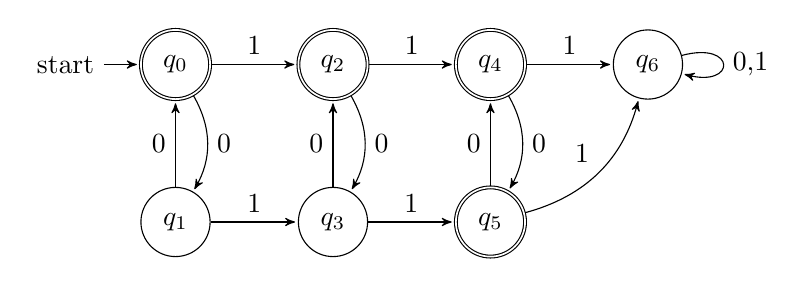
\begin{tikzpicture}[>=stealth',shorten >=1pt,auto,node distance=2cm]
 
% define the states in the machine
  \node[initial, state, accepting]    (q0)
 {$q_0$};
  \node[state]     (q1) [below of=q0]
{$q_1$};
  \node[state, accepting]   (q2)   [right of=q0]  	    
{$q_2$};
  \node[state]   (q3)   [below of=q2]
{$q_3$};
  \node[state, accepting]   (q4)   [right of=q2]
{$q_4$};
  \node[state, accepting]   (q5)   [below of=q4]
{$q_5$};
  \node[state]   (q6)   [right of=q4]
{$q_6$};
  
% define the links
  \path[->] (q0) edge node {1}   (q2)
             edge [bend left]    node {0}   (q1)
        (q1) edge     node {1} 	(q3)
             edge         node {0}  (q0)
        (q2) edge         node {1}   (q4)
             edge [bend left]       node {0}   (q3)     
        (q3) edge         node {0}   (q2) 
             edge         node {1}   (q5)  
        (q4) edge         node {1}  (q6)
             edge [bend left]       node {0}   (q5)
        (q5) edge  [bend right]       node {1}   (q6)
             edge         node {0}   (q4)
        (q6) edge   [loop right] node {0,1} (q6);
        
                                    
 \end{tikzpicture}
\end{center}

\textbf{ 9  Use the  construction in the proof of Theorem 1.47 to give the state diagrams NFAs regconize the concatenatetion of the languages described in. }\\
\textbf{a. Exercise 1.6g and 1.6i }\\

\begin{center}
 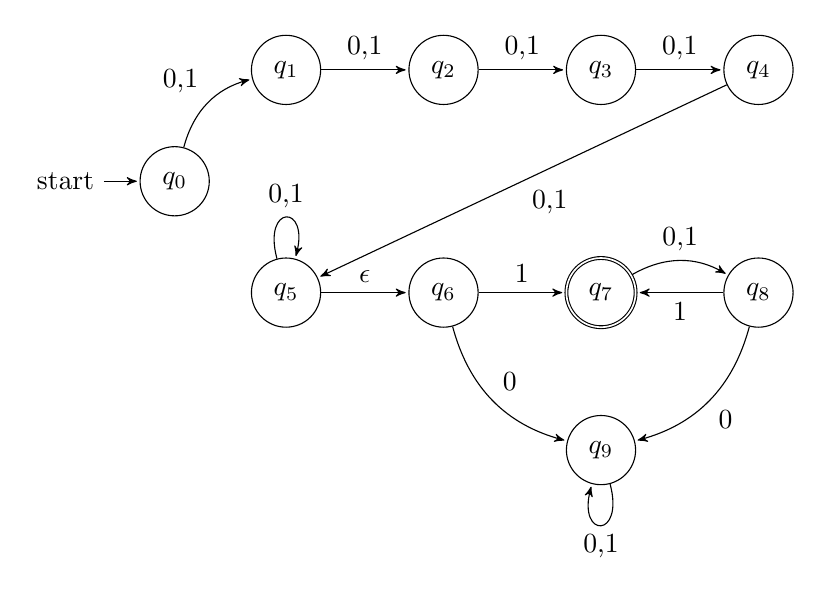
\begin{tikzpicture}[>=stealth',shorten >=1pt,auto,node distance=2cm]
 
% define the states in the machine
  \node[initial, state]    (q0) 
{$q_0$};
  \node[state]   (q1)   [above right of=q0]  	    
{$q_1$};
  \node[state]    (q2)  [right of=q1]
{$q_2$};
  \node[state]   (q3)   [right of=q2]  	    
{$q_3$};
  \node[state]   (q4)  [right of=q3]
{$q_4$};
  \node[state]   (q5)   [below right of=q0]  	    
{$q_5$};
  \node[state]    (q6)  [right of=q5]
{$q_6$};
  \node[state, accepting]   (q7)   [right of=q6]  	    
{$q_7$};
  \node[state]    (q8) [right of=q7]
{$q_8$};
  \node[state]    (q9) [below of=q7]
{$q_9$};
  
% define the links
  \path[->] (q0) edge [bend left] node {0,1} (q1)
               
        (q1) edge   node {0,1} (q2)
             
        (q2) edge   node {0,1}  (q3)
             
        (q3) edge   node {0,1}  (q4)
             
        (q4) edge    node {0,1}  (q5)
             
        (q5) edge  [loop above] node {0,1}  (q5)
             edge  node {$\epsilon$}   (q6)
        (q6) edge  node {1}  (q7)
             edge  [bend right] node {0} (q9)
        (q7) edge  [bend left] node {0,1} (q8)
             
        (q8) edge   node {1} (q7)
             edge   [bend left] node {0}  (q9)
        (q9) edge [loop below] node {0,1} (q9);
                                         
 \end{tikzpicture}
\end{center}


\end{document}
